\documentclass[xetex,mathserif,serif]{beamer}
\usepackage{polyglossia}
\setdefaultlanguage[babelshorthands=true]{russian}
\usepackage{minted}
\usepackage{tabu}

\useoutertheme{infolines}

\usepackage{fontspec}
\setmainfont{FreeSans}
\newfontfamily{\russianfonttt}{FreeSans}

\setbeamertemplate{blocks}[rounded][shadow=false]

\setbeamercolor*{block title alerted}{fg=red!50!black,bg=red!20}
\setbeamercolor*{block body alerted}{fg=black,bg=red!10}

\tabulinesep=1.2mm

\title{Контейнеры и генерики}
\author{Юрий Литвинов}
\date{3}

\begin{document}

	\frame{\titlepage}

	\begin{frame}
		\frametitle{Интерфейсы контейнеров}
		\begin{columns}
			\begin{column}{0.65\textwidth}
				\begin{itemize}
					\item IEnumerable --- штука, из которой можно последовательно получать элементы
					\item ICloneable --- штука, от которой можно делать глубокую копию
					\item ICollection --- абстрактная коллекция
					\item IDictionary --- расширение ICollection, абстрактный словарь
					\item IList --- расширение ICollection, коллекция, к элементам которой можно обращаться по индексу
				\end{itemize}
			\end{column}
			\begin{column}{0.3\textwidth}
				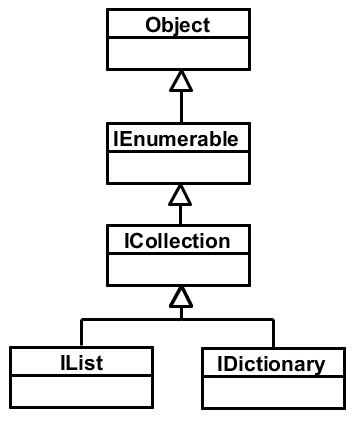
\includegraphics[width=\textwidth]{interfaces.png}
			\end{column}
		\end{columns}
	\end{frame}

	\begin{frame}[fragile]
		\frametitle{Энумератор}
		\begin{itemize}
			\item Абстрагирует обход коллекции, не может её модифицировать
			\item Реализует интерфейс IEnumerator
			\begin{itemize}
				\item Свойство Current
				\begin{itemize}
					\item Изначально --- перед первым элементом
				\end{itemize}
				\item MoveNext()
				\begin{itemize}
					\item Возвращает false после последнего элемента
				\end{itemize}
				\item Reset()
				\begin{itemize}
					\item Можно не реализовывать, тогда кидает NotSupportedException
				\end{itemize}
			\end{itemize}
			\item Компилятор знает про IEnumerable:
			\begin{minted}{csharp}
foreach (var i in list) { 
    Console.Write(i); 
}
			\end{minted}
			\item Инвалидируется при изменении коллекции (но Current продолжает работать)
		\end{itemize}
	\end{frame}

	\begin{frame}
		\frametitle{Негенериковые коллекции}
		\begin{itemize}
			\item ArrayList, реализует IList, ICollection, IEnumerable, ICloneable
			\item BitArray,  реализует ICollection, IEnumerable, ICloneable
			\item Hashtable, реализует IDictionary, ICollection, IEnumerable, ICloneable
			\item Queue, реализует ICollection, IEnumerable, ICloneable
			\item SortedList, реализует IDictionary, ICollection, IEnumerable, ICloneable
			\item Stack, реализует ICollection, IEnumerable, ICloneable
		\end{itemize}
	\end{frame}

	\begin{frame}[fragile]
		\frametitle{Почему негенериковые коллекции --- плохо}
		\begin{itemize}
			\item boxing/unboxing
			\begin{itemize}
				\item \mintinline{csharp}|list.Add(1);|
			\end{itemize}
			\item Типобезопасность
			\begin{itemize}
				\item \mintinline{csharp}|list.Add(1);|
				\item \mintinline{csharp}|list.Add("hello");|
			\end{itemize}
			\item Понижающие касты
			\begin{itemize}
				\item \mintinline{csharp}|var str = list[1] as string;|
			\end{itemize}
			\item Поэтому придумали генерики:
			\begin{minted}{csharp}
var list = new List<string>();
list.Add("hello");
var str = list[0];
			\end{minted}
			\begin{itemize}
				\item Так обычно пишут в книгах <<C\# для суперпрофессионалов>>, но это не совсем правда...
			\end{itemize}
		\end{itemize}
	\end{frame}

	\begin{frame}
		\frametitle{Полиморфизм}
		\begin{itemize}
			\item Ad-hoc
			\begin{itemize}
				\item Перегрузка
				\item Приведение
			\end{itemize}
			\item Универсальный
			\begin{itemize}
				\item Полиморфизм подтипов (сабтайпинг, наследование)
				\begin{itemize}
					\item 1..10 --- подынтервал 1..100, следовательно, подтип
					\item Принцип подстановки Лисков
				\end{itemize}
				\item Параметрический полиморфизм
				\begin{itemize}
					\item \mintinline{fsharp}|id: x: 'T -> x: 'T|
					\item \mintinline{fsharp}|id<int>(2)|
					\item \mintinline{fsharp}|id<string>("Cthulhu fhtagn!")|
					\item \mintinline{fsharp}|List<'T>| --- набор параметрически полиморфных функций
				\end{itemize}
			\end{itemize}
		\end{itemize}
	\end{frame}

	\begin{frame}
		\frametitle{Типы}
		\begin{itemize}
			\item Элементарные типы
			\item Конструкторы типов
			\begin{itemize}
				\item Подъязык для описания сложных типов
			\end{itemize}
			\item Структурное равенство и равенство по имени
			\item Выражения над типами
			\begin{itemize}
				\item Генерик --- это функция, принимающая набор параметров-типов и возвращающая тип
				\item На самом деле, функтор над категорией типов
			\end{itemize}
		\end{itemize}

		Подробности: Cardelli, Luca, and Peter Wegner. "On understanding types, data abstraction, and polymorphism." ACM Computing Surveys (CSUR) 17.4 (1985): pp. 471-523.
	\end{frame}

	\begin{frame}[fragile]
		\frametitle{Генерики в .NET}
		\begin{itemize}
			\item System.Collections.Generic
			\begin{minted}{csharp}
List<string> listOfStrings = new List<string>();
			\end{minted}
			\item Не требуют исходного кода генерика
			\begin{itemize}
				\item Информация о параметрах-типах есть в байт-коде
			\end{itemize}
			\item Не выполняют boxing, если параметр-тип --- тип-значение
			\begin{itemize}
				\item Для каждого параметра типа-значения при инстанциировании порождается новый код (как в C++)
				\item Для каждого параметра ссылочного типа байт-код переиспользуется (как в Java)
				\begin{itemize}
					\item Но не происходит стирание
				\end{itemize}
			\end{itemize}
		\end{itemize}

		Генерик-методы:
		\begin{minted}{csharp}
nt[] myInts = {1, 5, 2, 8, 4};
Array.Sort<int>(myInts);
		\end{minted}
	\end{frame}

	\begin{frame}[fragile]
		\frametitle{Свои генерик-методы}
		\begin{minted}{csharp}
static void Swap(ref int a, ref int b)
{
    int temp = a;
    a = b;
    b = temp;
}
		\end{minted}
		\hspace{2cm} $\Downarrow$
		\begin{minted}{csharp}
static void Swap<T>(ref T a, ref T b)
{
   T temp = a;
   a = b;
   b = temp;
}
		\end{minted}
	\end{frame}

	\begin{frame}[fragile]
		\frametitle{Использование}
		\begin{minted}{csharp}
int a = 10, b = 90;
Swap<int>(ref a, ref b);

string s1 = "Hello", s2 = "There";
Swap<string>(ref s1, ref s2);

bool b1 = true, b2 = false;
Swap(ref b1, ref b2);
		\end{minted}
	\end{frame}

	\begin{frame}[fragile]
		\frametitle{Генерик-классы}
		\begin{tiny}
			\begin{minted}{csharp}
public class Point<T>
{
   private T xPos;
   private T yPos;

   public Point(T xVal, T yVal)
   {
       xPos = xVal;
       yPos = yVal;
   }
   
   public T X
   {
       get { return xPos; }
       set { xPos = value; }
   }

   public override string ToString()
       => string.Format("[{0}, {1}]", xPos, yPos);

   public void ResetPoint()
   {
       xPos = default(T);
       yPos = default(T);
   }
}
			\end{minted}
		\end{tiny}
	\end{frame}

	\begin{frame}[fragile]
		\frametitle{Использование}
		\begin{minted}{csharp}
Point<int> p = new Point<int>(10, 10);
Point<double> p2 = new Point<double>(5.4, 3.3);

var p = new Point<int>(10, 10);
var p2 = new Point<double>(5.4, 3.3);
		\end{minted}
	\end{frame}

	\begin{frame}[fragile]
		\frametitle{Генерики и вложенные классы}
		\center{\textcolor{red}{TODO}}
		\begin{minted}{csharp}
		\end{minted}
	\end{frame}

	\begin{frame}[fragile]
		\frametitle{Ограничения}
		\begin{minted}{csharp}
public class MyGenericClass<T> where T : new()
public class MyGenericClass<T> where T : new(), class
public class MyGenericClass<T, U> 
    where T : new() 
    where U: class
		\end{minted}

		Доступные ограничения:
		\begin{itemize}
			\item \mintinline{csharp}|where T : struct|
			\item \mintinline{csharp}|where T : class|
			\item \mintinline{csharp}|where T : new()|
			\item \mintinline{csharp}|where T : NameOfBaseClass|
			\item \mintinline{csharp}|where T : NameOfInterface|
		\end{itemize}
	\end{frame}

	\begin{frame}[fragile]
		\frametitle{Вариантность}
		\begin{minted}{csharp}
public void f(Tuple<object, object> x)
{
    ...
}

f(new Tuple<object, object>(apple1, apple2));
f(new Tuple<Apple, Apple>(apple1, apple2));  // Ошибка компиляции
		\end{minted}
		\vspace{3mm}
		Чтобы нельзя было делать так:
		\begin{minted}{csharp}
public void f(Tuple<object, object> x)
{
    x.Item1 = new Battleship();
}
		\end{minted}
	\end{frame}

		\begin{frame}[fragile]
		\frametitle{Виды вариантности}
		\begin{footnotesize}
			\begin{itemize}
				\item \textbf{Ковариантность} --- A $\leq$ B => G<A> $\leq$ G<B>
				\begin{minted}{csharp}
void PrintAnimals(IEnumerable<Animal> animals) {
    for (var animal in animals)
      Console.WriteLine(animal.Name);
}
				\end{minted}
				--- IEnumerable<любой наследник Animal> тоже ок, IEnumerable ковариантен
				\item \textbf{Контравариантность} --- A $\leq$ B => G<B> $\leq$ G<A>
				\begin{minted}{csharp}
void CompareCats(IComparer<Cat> comparer) {
    var cat1 = new Cat("Otto");
    var cat2 = new Cat("Troublemaker");
    if (comparer.Compare(cat2, cat1) > 0) 
        Console.WriteLine("Troublemaker wins!");
}
				\end{minted}
				--- IComparer<любой предок Cat> тоже ок, IComparer контравариантен
				\item \textbf{Инвариантность} --- A $\leq$ B => G<A> и G<B> никак не связаны
				\begin{itemize}
					\item Пример с Tuple выше
				\end{itemize}
			\end{itemize}
		\end{footnotesize}
	\end{frame}

	\begin{frame}[fragile]
		\frametitle{Ковариантность массивов}
		\begin{minted}{csharp}
string[] a = new string[1];
object[] b = a;
b[0] = 1;
		\end{minted}
		--- System.ArrayTypeMismatchException, ошибка времени выполнения!
	\end{frame}

	\begin{frame}[fragile]
		\frametitle{Вариантность функциональных типов}
		\framesubtitle{Контравариантность по типам аргументов}
		\begin{minted}{csharp}
public class A
{
    public static void f(Func<string, object> a)
    {
        a("1");
    }
}
...
Func<object, object> b = x => x.ToString();
A.f(b);
		\end{minted}
	\end{frame}

	\begin{frame}[fragile]
		\frametitle{Вариантность функциональных типов}
		\framesubtitle{Ковариантность по возвращаемому значению}
		\begin{minted}{csharp}
Func<Object, ArgumentException> fn1 = null;
Func<Object, Exception> fn2 = fn1;
		\end{minted}

		Обратите внимание, ref-параметры сразу делают функцию инвариантной
	\end{frame}

	\begin{frame}[fragile]
		\frametitle{Явное указание вариантности для интерфейсов}
		\begin{minted}{csharp}
public interface IContainer<out T>
{
   T GetItem();
}


public interface IContainer<out T>
{
   void SetItem(T item);  // ошибка компиляции
   T GetItem();
}
		\end{minted}
	\end{frame}

	\begin{frame}
		\frametitle{Подробности}
		Взгляд на генерики и вариантность с точки зрения теории категорий:

		\href{http://tomasp.net/blog/variance-explained.aspx/}{http://tomasp.net/blog/variance-explained.aspx/}
	\end{frame}

\end{document}
